\section{Stereo Vision}
As detailed in section \ref{subsec:Camera_Model}, when converting from 3D to 2D we lose the depth information. However, with two images + some geometry we can potentially recover this information, as seen in the below image: 
\begin{figure}[H]
    \centering
    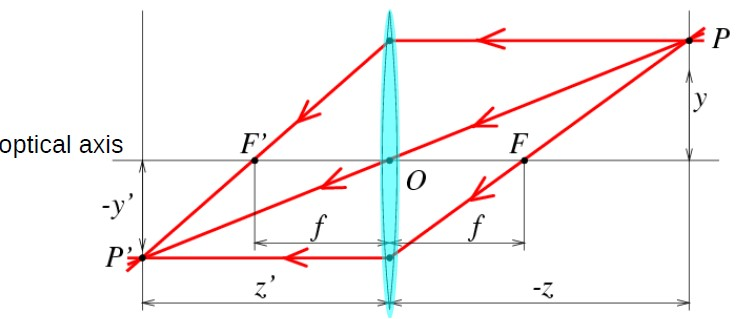
\includegraphics[width = \textwidth]{Images/Thin_Lens_Diagram} % Left vs right cameras
\end{figure}
By recovering depth information, we can use this to segment objects or recover/record the 3D shape of an object. 

\subsection{Co-Planar Cameras}
Two cameras with co-planar image planes (represented in front of the camera for convenience), same focal length, at the same height and parallel optical axes:
\begin{figure}[H]
    \centering
    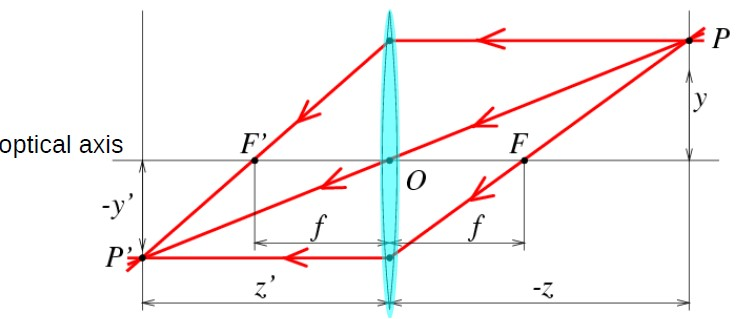
\includegraphics[width = \textwidth]{Images/Thin_Lens_Diagram} %Co-planar cameras
\end{figure}
The images are formed on the virtual planes at ($x_L,y_L$) and ($x_R,y_R$) for the left/right images respectively. Using the camera model equations (and assuming the image co-ordinate axes have (0,0) in the centre for convenience), we obtain the following for a scene point (x,y,z) (using $O_L$ as a reference):
\begin{align}
    x_L &= f_L \cdot \frac{x}{z} &&(f_L = f_R) \nonumber\\
    y_L &= f_L \cdot \frac{y}{z} = y_R &&(\text{The image planes are at the same height, so }y_L = y_R) \nonumber\\
    x_R &= f_L \cdot \frac{(x-B)}{z} && \dagger \nonumber\\
    Disparity = d &=  x_L - x_R = f_L \cdot \frac{x}{z} - &&f_L \cdot \frac{(x-B)}{z} = f \cdot \frac{B}{z}
\end{align}
$\dagger$ B is the x-difference between the two cameras. As (x,y,z) is in terms of $O_L$, B is subtracted to convert to $O_R$'s co-ordinate system.\\

From the above system of equations, we can see that depth$\propto\frac{1}{disparity}$ - B is known, d can be observed form the images, so z (depth) can be calculated given the two images. If B isn't known, then we can still calculate relative depth. d is simply the difference vector between two corresponding points in the images (horizontal for coplanar cameras). 

\subsection{Stereo Correspondence}
If z (depth) $>>$ B(baseline camera distance), then most points will be visible in both images and corresponding points will be similar - it's still not an easy problem, but there are several constraints we can make use of:
\begin{enumerate}
    \item Epipolar Constraint - for co-planar cameras, the y-coordinate is the same so it's reduced to a 1D search 
    \item $Disparity_{max} = f \cdot \frac{B}{Depth_{min}}$
    \item Neighbouring points along continuous surfaces will have similar disparities. At sudden discontinuities of depth, this no longer holds
    \item Guaranteed Uniqueness - Each point can only map to one point in the other image. The exception is a surface inclined along the line of sight for one camera (e.g. a cuboid directly pointing at one camera) - this will have one point in this camera's image, but multiple in the other camera
    \item Ordering - Matching points on \emph{Epipolar Lines} (corresponding co-planar lines, in this case lines with the same y axis) will be in the same order - this doesn't work at depth discontinuities. 
\end{enumerate}
\begin{figure}[H]
    \centering
    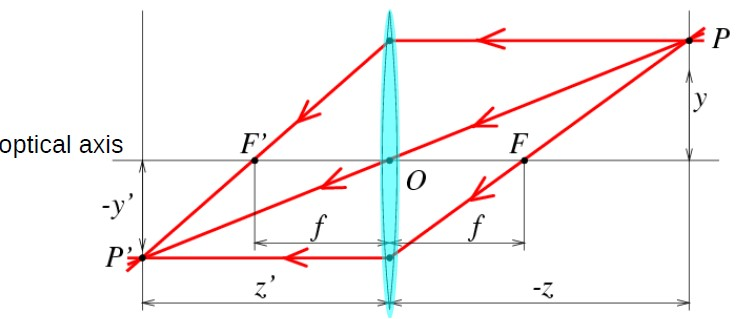
\includegraphics[width = \textwidth]{Images/Thin_Lens_Diagram} % Depth discontinutities
\end{figure}
Sometimes we can't find corresponding points due to occlusion or different Fields Of View (depth can only be recovered where the FoV overlap). The closer the cameras, the larger the overlapping FoV, but the larger error in depth estimates ($depth \propto \frac{1}{baselineDistance})$. 

\subsection{Non-Coplanar Cameras}
The cameras/image planes are angled towards each other - the \emph{vergence angle} ($\theta$) is the angle between the optical axes. Disparity is measured using angles rather than distance ($\alpha_L - \alpha_R$) - it's zero at the \emph{fixation point}(where the optical axes meet) and where rays at equal angles intercept (This curve is called the \emph{horopter)}, $>0$ further than the horopter and $<0$ closer than the horopter. 
\begin{figure}[H]
    \centering
    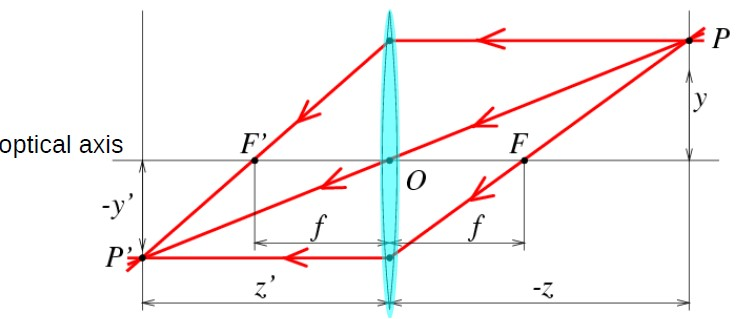
\includegraphics[width = \textwidth]{Images/Thin_Lens_Diagram} % Non-coplanar cameras
\end{figure}

Eyes are an example of non-coplanar cameras that can adjust the vergence angle. The fixation point is projected to the fovea, points on the horopter are at an equal distance from the fovea in each eye, points further fall outside the fovea on both sides (crossed) and points closer fall inside on both side (uncrossed). Some neurons are tuned to disparity, and can calculate the depth of image points. 
\begin{figure}[H]
    \centering
    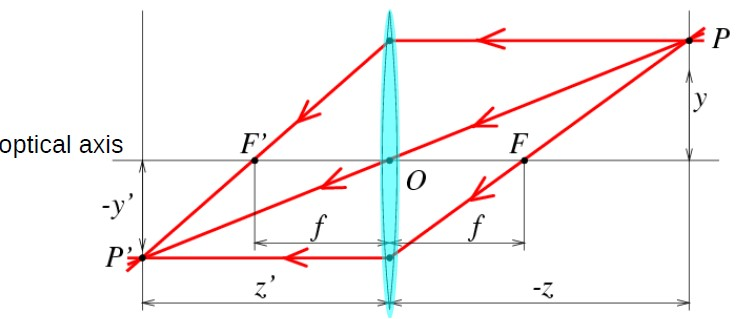
\includegraphics[width = \textwidth]{Images/Thin_Lens_Diagram} % Eye disparities
\end{figure}

\subsubsection{Epipolar Geometry}
Though the image planes are no longer co-planar, corresponding points still appear on the same lines (though no longer horizontal). These epipolar lines are the intersection of the \emph{epipolar plane}(plane passing through a scene point and both optic centers) with the image planes. \emph{Conjugated Epipolar lines} are the epipolar lines generated from the same epipolar plane - corresponding points always lie on conjugated epipolar lines.\\

All epipolar lines meet the \emph{baseline} (line between the two camera centres) at the \emph{epipole}(intersection of the image plane with the baseline)(projection of the centre of one camera in the image plane of the other camera, nor usually shown).\\

\emph{Rectification} is adjusting the images to make the epipolar lines horizontal.

\subsubsection{Calculating the Depth}
Unlike in co-planar cameras, there is no simple formula. Depth can be calculated using triangulation (determining the intersection of corresponding view lines) or rectifying the image then using the regular formula - both require knowledge of internal and external camera parameters).

\subsection{Depth Cues}
\subsubsection{Binocular (two images)}
\begin{description}
    \item[Disparity] The difference in position of an object between the two images
    \item[Accommodation] In the eye, how much the lens has been adjusted (to obtain f)
    \item[Convergence] The vergence angle - known for cameras, can be calculated from muscle movements for eyes
\end{description}

\subsubsection{Monocular (One Image)}
\begin{description}
    \item[Interposition] If an object occludes another, we assume it's in front of it (uses grouping cues/closed contours to see if it's infront or simply an odd shape)
    \item[Size Familiarity] If we see two objects identical other than size, then we assume the smaller is further away
    \item[Texture Gradients] Textures get closer together/smaller with depth
    \item[Linear Perspective] Parallel lines converge at infinity - these can provide cues to depth/size of objects
    \item[Aerial Perspective] Light scatters as it travels, so distant objects are blurred/less colourful (Reduced contrast/saturation)
    \item[Shading] position of light/shadows gives depth cues. The brain assumes light comes from above, so objects with longer shadows must be taller
\end{description}

\subsubsection{Motion-Induced}
\begin{description}
    \item[Motion Parallax] Speed/direction of image motion with camera/eye movement. Objects closer than the fixation point move in the \emph{opposite direction}, objects further move faster
    \item[Optic Flow] As the observer moves forwards/backwards, the image expands/contracts. The closer the point the the camera, the faster it moves.
    \item[Accretion/Deletion] Parts of the image appear/disappear (due to occlusion) as the observer moves, which gives depth cues
    \item[Kinetic Depth] Movement of the object can induce a 3D perception
\end{description}




